\documentclass{standalone}

% font set
\usepackage{ctex}
\usepackage{fontspec}
\usepackage[sc]{mathpazo}
\usepackage{anyfontsize}

\setmainfont{SourceSerif4-Regular.ttf}[%
    Path = ../../fonts/,
    BoldFont = SourceSerif4-Bold.ttf,
    ItalicFont = SourceSerif4-It.ttf,
    BoldItalicFont = SourceSerif4-BoldIt.ttf
]
\setCJKmainfont[%
    Path = ../../fonts/,
    BoldFont=SourceHanSansSC-Medium.otf,
    ItalicFont=gkai00mp-2.ttf%
]{SourceHanSansSC-Normal.otf}

% colors
\usepackage[dvipsnames]{xcolor}
\definecolor{pku-red}{RGB}{139,0,18}
\usepackage{colortbl}
\newcommand{\light}[1]{\textcolor{Orchid}{#1}}
\newcommand{\contrastlight}[1]{\textcolor{TealBlue}{#1}}

\usepackage[normalem]{ulem}

\usepackage{makecell}

% math package
\let\Bbbk\relax
\usepackage{amsmath}
\usepackage{mathrsfs}
\usepackage{amssymb}
\usepackage{amsfonts}
\usepackage{stmaryrd}
\usepackage{latexsym}
\usepackage{extarrows}
\SetSymbolFont{stmry}{bold}{U}{stmry}{m}{n}
\allowdisplaybreaks[3]


% math notations
\newcommand{\LHS}{\mathrm{LHS}}
\newcommand{\RHS}{\mathrm{RHS}}
\newcommand{\Z}{\mathbb{Z}}
\newcommand{\N}{\mathbb{N}}
\newcommand{\R}{\mathbb{R}}
\newcommand{\Q}{\mathbb{Q}}
\newcommand{\C}{\mathbb{C}}
\newcommand{\E}{\mathbb{E}}
\renewcommand{\O}{\mathcal{O}}
\newcommand{\id}{\mathrm{id}}
\DeclareMathOperator*{\Span}{Span}
\DeclareMathOperator*{\im}{Im}
\DeclareMathOperator*{\rank}{rank}
\DeclareMathOperator*{\card}{card}
\DeclareMathOperator*{\grad}{grad}
\DeclareMathOperator*{\argmax}{argmax}
\DeclareMathOperator*{\epi}{epi}
\DeclareMathOperator*{\maximize}{maximize}
\DeclareMathOperator*{\minimize}{minimize}
\renewcommand{\d}{\mathrm{d}}
\newcommand{\Pow}{\mathcal{P}}
\newcommand{\cov}{\mathsf{Cov}}
\newcommand{\var}{\mathsf{Var}}
\newcommand{\Nor}{\mathcal{N}}
\newcommand{\U}{\mathcal{U}}
\renewcommand{\t}{\mathsf{T}}
\newcommand{\T}{\top}
\newcommand{\F}{\bot}
\newcommand{\norm}[1]{\left\|#1\right\|}
\newcommand{\inner}[2]{\left\langle{#1},{#2}\right\rangle}
\newcommand{\e}{\mathrm{e}}
\newcommand{\const}{\mathrm{const}}
\newcommand{\scB}{\mathscr{B}}
\newcommand{\scF}{\mathscr{F}}
\newcommand{\G}{\mathscr{G}}
\newcommand{\Exp}{\mathsf{Exp}}
\newcommand{\DExp}{\mathsf{DExp}}
\newcommand{\Lap}{\mathsf{Lap}}
\newcommand{\calP}{\mathcal P}
\newcommand{\calS}{\mathcal S}
\newcommand{\calF}{\mathcal F}
\newcommand{\calM}{\mathcal M}
\newcommand{\KL}{\mathrm{KL}}
\newcommand{\ReLU}{\mathsf{ReLU}}
\newcommand{\val}{\mathsf{val}}

% plots
\usepackage{tikz}
\usetikzlibrary{arrows}
\usetikzlibrary{arrows.meta,positioning,calc,3d}
\usepackage{tikz-3dplot}
\usepackage{pgfplots}
\pgfplotsset{compat=newest}

\newcommand{\drawX}[2]{\draw[line width=2, Orchid] (#1+0.2, #2+0.8) -- (#1+0.8, #2+0.2); \draw[line width=2, Orchid] (#1+0.2, #2+0.2) -- (#1+0.8, #2+0.8);}

\newcommand{\drawO}[2]{\draw[line width=2, TealBlue] (#1+0.5, #2+0.5) circle(0.3);}

\newcommand{\drawGrid}{
    \draw[line width=2] (0,1) -- (3,1);
    \draw[line width=2] (0,2) -- (3,2);
    \draw[line width=2] (1,0) -- (1,3);
    \draw[line width=2] (2,0) -- (2,3);
}

\begin{document}

\begin{tikzpicture}[
    level distance=3.5cm,
    level 2/.style={sibling distance=2.5cm},
    sibling distance=5.5cm,
    edge from parent/.style={draw,thick},
    every node/.style={scale=0.7,align=center}
]
\node (0) {\begin{tikzpicture}
    % 画井字棋的网格
    \drawGrid
    \drawO{0}{2}
    \drawO{0}{0}
    \drawO{1}{2}
    \drawX{1}{0}
    \drawX{1}{1}
    \drawX{2}{2}
\end{tikzpicture}}

child {node (10) {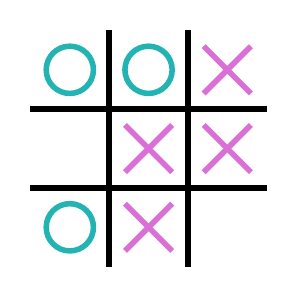
\begin{tikzpicture}
    % 画井字棋的网格
    \drawGrid
    \drawO{0}{2}
    \drawO{0}{0}
    \drawO{1}{2}
    \drawX{1}{0}
    \drawX{1}{1}
    \drawX{2}{2}
    \drawX{2}{1}
\end{tikzpicture}}
child {node (100) {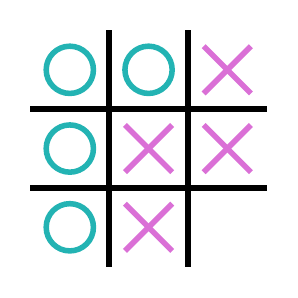
\begin{tikzpicture}
    % 画井字棋的网格
    \drawGrid
    \drawO{0}{2}
    \drawO{0}{0}
    \drawO{1}{2}
    \drawO{0}{1}
    \drawX{1}{0}
    \drawX{1}{1}
    \drawX{2}{2}
    \drawX{2}{1}
\end{tikzpicture}}}
child {node (101) {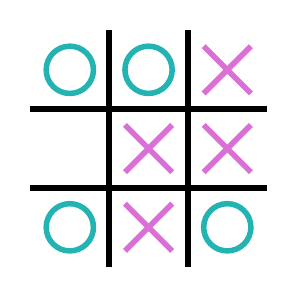
\begin{tikzpicture}
    % 画井字棋的网格
    \drawGrid
    \drawO{0}{2}
    \drawO{0}{0}
    \drawO{1}{2}
    \drawO{2}{0}
    \drawX{1}{0}
    \drawX{1}{1}
    \drawX{2}{2}
    \drawX{2}{1}
\end{tikzpicture}}
child {node (1011) {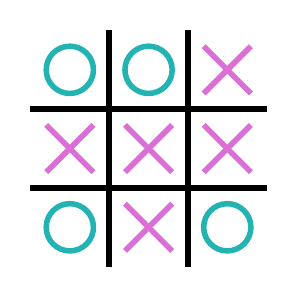
\begin{tikzpicture}
    % 画井字棋的网格
    \drawGrid
    \drawO{0}{2}
    \drawO{0}{0}
    \drawO{1}{2}
    \drawO{2}{0}
    \drawX{1}{0}
    \drawX{1}{1}
    \drawX{2}{2}
    \drawX{2}{1}
    \drawX{0}{1}
\end{tikzpicture}}}}}
child {node (11) {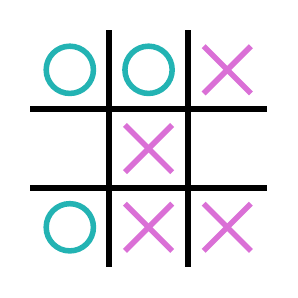
\begin{tikzpicture}
    % 画井字棋的网格
    \drawGrid
    \drawO{0}{2}
    \drawO{0}{0}
    \drawO{1}{2}
    \drawX{1}{0}
    \drawX{1}{1}
    \drawX{2}{2}
    \drawX{2}{0}
\end{tikzpicture}}
child {node (110) {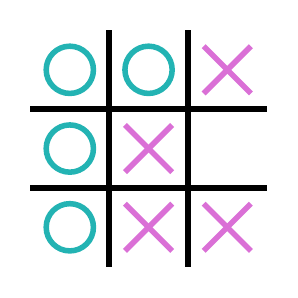
\begin{tikzpicture}
    % 画井字棋的网格
    \drawGrid
    \drawO{0}{2}
    \drawO{0}{0}
    \drawO{1}{2}
    \drawO{0}{1}
    \drawX{1}{0}
    \drawX{1}{1}
    \drawX{2}{2}
    \drawX{2}{0}
\end{tikzpicture}}}
child {node (111) {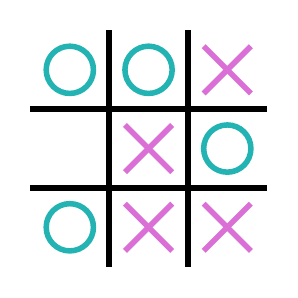
\begin{tikzpicture}
    % 画井字棋的网格
    \drawGrid
    \drawO{0}{2}
    \drawO{0}{0}
    \drawO{1}{2}
    \drawO{2}{1}
    \drawX{1}{0}
    \drawX{1}{1}
    \drawX{2}{2}
    \drawX{2}{0}
\end{tikzpicture}}
child {node (1110) {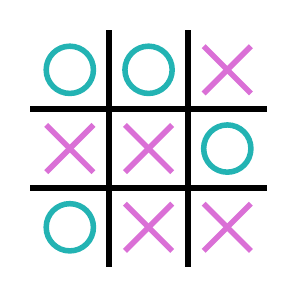
\begin{tikzpicture}
    % 画井字棋的网格
    \drawGrid
    \drawO{0}{2}
    \drawO{0}{0}
    \drawO{1}{2}
    \drawO{2}{1}
    \drawX{1}{0}
    \drawX{1}{1}
    \drawX{2}{2}
    \drawX{2}{0}
    \drawX{0}{1}
\end{tikzpicture}}}}}
child {node (12) {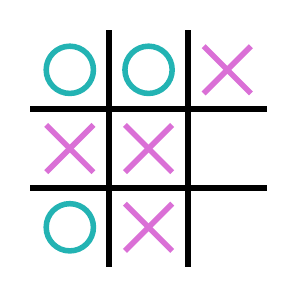
\begin{tikzpicture}
    % 画井字棋的网格
    \drawGrid
    \drawO{0}{2}
    \drawO{0}{0}
    \drawO{1}{2}
    \drawX{1}{0}
    \drawX{1}{1}
    \drawX{2}{2}
    \drawX{0}{1}
\end{tikzpicture}}
child {node (120) {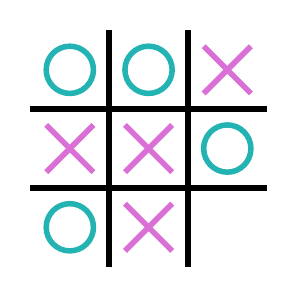
\begin{tikzpicture}
    % 画井字棋的网格
    \drawGrid
    \drawO{0}{2}
    \drawO{0}{0}
    \drawO{1}{2}
    \drawO{2}{1}
    \drawX{1}{0}
    \drawX{1}{1}
    \drawX{2}{2}
    \drawX{0}{1}
\end{tikzpicture}}
child {node (1201) {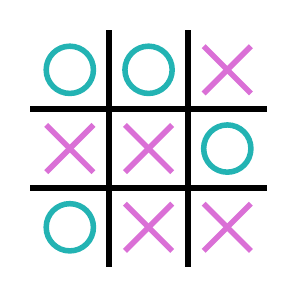
\begin{tikzpicture}
    % 画井字棋的网格
    \drawGrid
    \drawO{0}{2}
    \drawO{0}{0}
    \drawO{1}{2}
    \drawO{2}{1}
    \drawX{1}{0}
    \drawX{1}{1}
    \drawX{2}{2}
    \drawX{0}{1}
    \drawX{2}{0}
\end{tikzpicture}}}}
child {node (121) {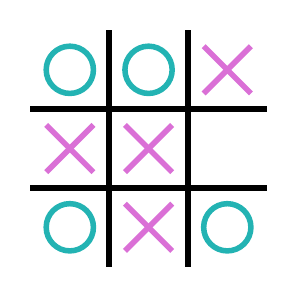
\begin{tikzpicture}
    % 画井字棋的网格
    \drawGrid
    \drawO{0}{2}
    \drawO{0}{0}
    \drawO{1}{2}
    \drawO{2}{0}
    \drawX{1}{0}
    \drawX{1}{1}
    \drawX{2}{2}
    \drawX{0}{1}
\end{tikzpicture}}
child {node (1111) {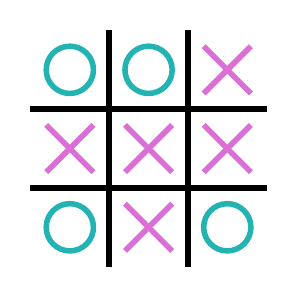
\begin{tikzpicture}
    % 画井字棋的网格
    \drawGrid
    \drawO{0}{2}
    \drawO{0}{0}
    \drawO{1}{2}
    \drawO{2}{0}
    \drawX{1}{0}
    \drawX{1}{1}
    \drawX{2}{2}
    \drawX{0}{1}
    \drawX{2}{1}
\end{tikzpicture}}}}};

\node[scale=2,xshift=2cm,Orchid] at (0) {X的轮次};
\node[scale=2,xshift=-1cm,Orchid] at (0) {$0$};
\node[scale=2,yshift=1cm,Orchid] at (10) {$-1$};
\node[scale=2,yshift=1cm,xshift=0.5cm,Orchid] at (11) {$-1$};
\node[scale=2,yshift=1cm,Orchid] at (12) {$0$};
\node[scale=2,yshift=1cm,Orchid] at (100) {$-1$};
\node[scale=2,yshift=1cm,Orchid] at (101) {$+1$};
\node[scale=2,yshift=1cm,Orchid] at (110) {$-1$};
\node[scale=2,yshift=1cm,Orchid] at (111) {$0$};
\node[scale=2,yshift=1cm,Orchid] at (120) {$0$};
\node[scale=2,yshift=1cm,Orchid] at (121) {$+1$};
\node[scale=2,yshift=1cm,xshift=0.5cm,Orchid] at (1011) {$+1$};
\node[scale=2,yshift=1cm,xshift=0.5cm,Orchid] at (1110) {$0$};
\node[scale=2,yshift=1cm,xshift=0.5cm,Orchid] at (1111) {$0$};
\node[scale=2,yshift=1cm,xshift=0.5cm,Orchid] at (1201) {$+1$};
\end{tikzpicture}

\end{document}
